% Adjust these for the path of the theme and its graphics, relative to this file
%\usepackage{beamerthemeFalmouthGamesAcademy}
\usepackage{../../beamerthemeFalmouthGamesAcademy}
\usepackage{multimedia}
\graphicspath{ {../../} }

\usepackage{textcomp}

% Default language for code listings
\lstset{language=Python, upquote=true,
        morekeywords={each,in,nullptr}
}

% For strikethrough effect
\usepackage[normalem]{ulem}
\usepackage{wasysym}
\usepackage{pdfpages}
\usepackage{epstopdf} % For EPS

% http://www.texample.net/tikz/examples/state-machine/
\usetikzlibrary{arrows,automata}

\newcommand{\modulecode}{COMP260}\newcommand{\moduletitle}{Distributed Systems}\newcommand{\sessionnumber}{5}

\setbeamertemplate{navigation symbols}{}

\newcommand{\fullbleed}[1]{
\begin{frame}[plain]
	\begin{tikzpicture}[remember picture, overlay]
		\node[at=(current page.center)] {
			\includegraphics[width=\paperwidth]{#1}
		};
	\end{tikzpicture}
\end{frame}
}

\newcommand{\picturepage}[2]{
\begin{frame}[plain]
	\begin{tikzpicture}[remember picture, overlay]
		\node[at=(current page.center)] {
			\includegraphics[width=\paperwidth]{#1}
		};
		\draw<1>[draw=none, fill=black, opacity=0.9] (-1,-5.2) rectangle (current page.south east);
		\node[draw=none,text width=0.96\paperwidth, align=right] at (5.5,-5.5) {\tiny{#2}};
	\end{tikzpicture}
\end{frame}
}

\newcommand{\notepicx}[5]{
\begin{frame}[plain]
	\begin{tikzpicture}[remember picture, overlay]
		\node[at=(current page.center)] {
			\includegraphics[width=\paperwidth]{#1}
		};
		\node[draw=none, fill=black, text width=#5\paperwidth] at ([xshift=#3, yshift=#4] current page.center) {\small{#2}};
	\end{tikzpicture}
\end{frame}
}

\newcommand{\notepic}[4]{
	\notepicx{#1}{#2}{#3}{#4}{0.4}
}

\begin{document}
\title{\sessionnumber: Introduction to Computing}
\subtitle{\modulecode: \moduletitle}

\frame{\titlepage} 

\begin{frame}
	\frametitle{Learning Outcomes}
	\begin{itemize}
		\item \textbf{Recognise THREE} of the key challenges associated with your first block of study
		\item \textbf{Identify} approaches to managing time
		\item \textbf{Recall} important theories about teamwork
		\item \textbf{Recall} important theories about learning computer programming
	\end{itemize}
\end{frame}


\part{Challenges in Higher Education}
\frame{\partpage}

\begin{frame}
	\frametitle{Challenges in the Transition to Higher Education}
	
	Students encounter many challenges when setting out on computing courses, however these are the three that I observe most often:
	
	\begin{itemize}
		\item Time management
		\item Teamwork
		\item Programming
	\end{itemize}
\end{frame}

\begin{frame}
	\frametitle{TwitterFall Activity}
		
	\begin{itemize}
		\item Self-organise into \textbf{THREE} groups
		\item Load a Twitter app, or login to Twitter on a PC
		\item Research and discuss tips on:
		\begin{itemize}			 
			\item \textbf{time management}
			\item \textbf{teamwork}
			\item \textbf{learning programming}
		\end{itemize}
		\item Tweet your tips!
	\end{itemize}

	\begin{itemize}
		\item You have 15 minutes
		\item Please use the hashtag for the module (i.e., \lstinline{\#comp110})
		\item Also please ensure you use the \lstinline{@} symbol to open and continue discussions
	\end{itemize}
\end{frame}

\part{Time Management}
\frame{\partpage}

\begin{frame}
	\frametitle{Common Pitfalls}
	
	Among others, common pitfalls include:
	
	\begin{itemize}
		\item Not setting a goal
		\item Failing to identify tasks that need doing
		\item Poor track of tasks done and tasks outstanding
		\item Poor prioritisation
		\item Lack of scheduling
		\item Not starting tasks immediately
	\end{itemize}

\end{frame}

\begin{frame}
	\frametitle{Common Pitfalls}
	
	Among others, common pitfalls include:
	
	\begin{itemize}
		\item Not committing to at least 40-hours per week
		\item Inability to say `no'
		\item Multi-tasking inefficiency
		\item Procastination
		\item Crunching
		\item Sleeping too much		
	\end{itemize}

\end{frame}
		
\begin{frame}
	\frametitle{Overcoming the Pitfalls}
	
	\begin{itemize}
		\item The trick is recognising the volume of work and planning ahead
		\item It is easier to motivate yourself to get small well-defined tasks out of the way, then to tackle nebulous and seemingly insurmountable tasks.
		\item Grasping a sense of flow and consistency is critically important	
	\end{itemize}

\end{frame}

\fullbleed{mayo-jar}

\fullbleed{covey-4-quadrants}

%\begin{frame}
%	\frametitle{Activity}
%	
%	On a calendar app, such as \url{http://teamup.com}, set-up:
%	
%	\begin{itemize}
%		\item Deadline dates for your assignments (from MyFalmouth)
%		\item The `formative' in-class deadlines (from MyTimetable)
%		\item Times that you plan to use for recreational activities
%		\item Times that you plan to use to do your coursework
%	\end{itemize}
%	
%	\vspace{2em}
%	
%	There is a shared calendar at: \url{https://teamup.com/ksdfj51dtrjd4n6wo2}
%	
%	\vspace{2em}
%	
%	You have 10 minutes. Finish in your own time.
%	
%\end{frame}

\part{Teamwork}
\frame{\partpage}

\begin{frame}
	\frametitle{Value of Collaboration}
	
	Games are made by teams of people working collaboratively, bringing people from different disciplines come together to make different kinds of contribution. 
	
	\vspace{1em}
	
	Advantages include:
	
	\begin{itemize}
		\item Fostering a mix of skills that go beyond the capabilities of a single individual
		\item Faster problem solving
		\item Broader range of experiences and learnings from which to generate ideas
		\item More person-hours enables teams to tackle more ambitious goals
	\end{itemize}
\end{frame}

\begin{frame}
	\frametitle{Value of Collaboration}
	
	Other advantages include:
	
	\begin{itemize}
		\item Organisational learning, sharing discoveries and insights across team members to increase productivity
		\item Sense of camaraderie and belonging aids motivation
		\item Mutual quality assurance and verification
		\item Robustness---support mechanisms and flexibility when life happens to get in the way
	\end{itemize}
\end{frame}

\begin{frame}
	\frametitle{Difficulties}
	
	At first, everyone finds working with other people challenging. Common difficulties include:
	
	\begin{itemize}
		\item Remembering names and individual differences
		\item Nobody trusting each other
		\item Differing vocabularies and contrasting perspectives
		\item Everyone is coming in with different personalities
		\item People have different beliefs and positions regarding the way things \textit{should} be done
		\item Members of the team will have different skills with varying levels of competence
		\item Emotional labour needed to forge relationships with new people 
	\end{itemize}
\end{frame}

\begin{frame}
	\frametitle{Expect Challenge}
	
	First-year teams always experience significant challenge! 
	
	\vspace{2em}
	
	Your team might fall apart and fail. If so, embrace the situation and reflect deeply---it's a learning experience (and you won't fail the course so don't worry)!
	
	\vspace{2em}
	
	This first block of study is about recognising points of failure and resolving conflicts. 
	It is your space to develop tolerance, coping mechanisms, new ways to communicate, and management skills.
\end{frame}

\begin{frame}
	\frametitle{Tuckman's Model}
	
	Teams go through various phases:
	
	\begin{itemize}
		\item Forming
		\item Storming
		\item Norming
		\item Performing
		\item Adjourning
	\end{itemize}
	
	You should \textbf{expect} conflicts and fall outs whilst \textit{storming}. Part of being a professional is developing professional conduct---not over-personalising criticisms and disagreeing with peers in a constructive and polite manner. For more insight, see: 
	
	\vspace{1em}	
	
	\url{http://faculty.wiu.edu/P-Schlag/articles/Stages_of_Small_Group_Development.pdf}
	
\end{frame}

\begin{frame}
	\frametitle{Belbin Roles---Thinkers}
	
	People have different role preferences. Some people are:
	
	\begin{itemize}
		\item \textbf{Plant}: Plants are creative, unorthodox and generators of ideas.
		\item \textbf{Monitor Evaluator}: fair and logical observers and judges of what is going on in the team
		\item \textbf{Specialist}: passionate about learning in their own particular field; as a result, they are likely to be a fountain of knowledge on a particular topic and will enjoy imparting this knowledge to others.
	\end{itemize}
	
\end{frame}

\begin{frame}
	\frametitle{Belbin Roles---Actioneers}
	
	People have different role preferences. Some people are:
	
	\begin{itemize}
		\item \textbf{Shaper}: a task-focused individual who pursues objectives with vigour.
		\item \textbf{Implementer}: takes their colleagues' suggestions and ideas and turns them into positive action.
		\item \textbf{Completer-Finisher}: a perfectionist and will often go the extra mile to make sure everything is `just right' and the things she or he delivers can be trusted to have been double-checked and then checked again.
	\end{itemize}
	
\end{frame}

\begin{frame}
	\frametitle{Belbin Roles---Socialisers}
	
	People have different role preferences. Some people are:
	
	\begin{itemize}
		\item \textbf{Co-ordinator}: the likely candidate for the chairperson of a team, since they have a talent for stepping back to see the big picture.
		\item \textbf{Teamworker}: the oil between the cogs that keep the machine that is the team running smoothly. They are good listeners and diplomats, talented at smoothing over conflicts and helping parties understand one another without becoming confrontational.
		\item \textbf{Resource Investigator}: gives a team a rush of enthusiasm at the start of the project by vigorously pursuing contacts and opportunities.
	\end{itemize}
	
\end{frame}

\begin{frame}
	\frametitle{Belbin's Inventory}
		
	\begin{itemize}
		\item Team composition matters---two people with preference for the same role will likely come into conflict
		\item Role preferences matter---e.g., people with a strong completer-finisher preference typically won't do well with early-stage ideation tasks, deploy a plant instead
		\item Utilise talent---let people play to their strengths, and value their contribution (don't neglect teamworkers)
		\item People have multiple preferences with varying strengths---some people are more versatile than others, but everyone makes critically important contributions
		\item Preferences can change over time
	\end{itemize}
	
\end{frame}

\begin{frame}
	\frametitle{Salas' Big-5 Model}
	
	In teams, it's important to openly communicate and develop strategies to support each other. Salas' approach focuses on those coordinating mechanisms associated with team effectiveness, indicating where you should focus your efforts:
	
	\begin{itemize}
		\item Closed-Loop Communication
		\item Mutual Trust
		\item Shared Mental Models
	\end{itemize}
	
\end{frame}

\begin{frame}
	\frametitle{Salas' Big-5 Model}
	\vspace{0.5em}
	
\begin{figure}[!tb]
\centering
\includegraphics[width=.55\textwidth]{five_team.eps}
\caption{Five-Factor Model of Team Effectiveness with Coordinating Mechanisms (from Salas, 2005)}
\label{fig:five-teamwork}
\end{figure}
	
\end{frame}

\begin{frame}
	\frametitle{Salas' Big-5 Model}
	
	In order to be effective as a team, you need to:
	
	\begin{itemize}
		\item Orient yourselves towards a shared goal
		\item Identify your coordinator(s) and monitor-evaluator(s) to establish leadership 
		\item Collectively devise an approach to mutual performance monitoring
		\item Develop back-up behaviours for when things go wrong
		\item Adapt
	\end{itemize}
	
	These typically have to be learned practically, and so we have the rest of the week to focus on these!
	
\end{frame}

\part{Learning Programming}
\frame{\partpage}

\begin{frame}
	\frametitle{Learning Programming}
	
	\begin{itemize}
		\item Games industry is fast-moving, rapdily adopting new technologies
		\item Programming languages and APIs change, so you will continue learning throughout your career
		\item A goal of this course is to facilitate your development as self-regulated learners
		\item Gradually, more independence across each year of study
		\item This is a science degree, which means you will become a producer of knowledge, not just a consumer of knowledge!
	\end{itemize}
\end{frame}

\begin{frame}
	\frametitle{Learning Programming}
	
	\begin{itemize}
		\item It isn't easy!
		\item Most of you will encounter programming anxiety
		\item Some will experience a sense of fear or a sense of hopelessness --- it is more common than you think
		\item Some will need more support than others --- this isn't a bad thing
		\item Everyone who puts in the time and effort will achieve mastery, eventually
	\end{itemize}
\end{frame}

\begin{frame}
	\frametitle{Key Learning Theories}
	
	\begin{itemize}
		\item Deliberate Practice
		\item Scaffolding and the Zone of Proximal Development
		\item Schema Development
		\item Cognitive Load
		\item Learning Edge Momentum
		\item Mindset
		\item Neuroplasticity
		\item Self-Determination
	\end{itemize}
\end{frame}

\fullbleed{deliberate_practice}

\begin{frame}
	\frametitle{Deliberate Practice}
	
	``\textbf{Attention to the task:} It is essential to pay fixed attention. The more a student's
	mind wanders, the less the rate of change. Even videogames require the subject to stay
	`locked in' to the content and the process.''
	
	 (Jensen, 2006, p. 82) 
	
\end{frame}

\begin{frame}
	\frametitle{Deliberate Practice}
	
	``\textbf{Low to moderate stress:} This variable is quite slippery because what is stressful
	for one may not be stressful for another. The bottom line is that the subject must perceive
	some choice or control over the task and the surrounding conditions. Otherwise, the stress 
	from that loss of control may neutralize the positive effects from the learning.''
	
	 (Jensen, 2006, p. 82) 
	
\end{frame}

\fullbleed{performance-pressure}

\fullbleed{zpd}

\fullbleed{schema_theory}

\fullbleed{cognitive_load}

\fullbleed{network_lem}

\begin{frame}
	\frametitle{Mindsets}
	
	Watch the video at:
	
	\vspace{1.5em}
		
	\url{https://www.dropbox.com/s/8wy1mbkud7n5ns3/Growth\%20vs\%20Fixed\%20Mindset.mp4?dl=0}
	
	\vspace{1em}
		
	(5 minutes)
	
\end{frame}

\fullbleed{mj_growth_mindset}

\begin{frame}
	\frametitle{Neuroplasticity}
	
	Medina (2008) demonstrates:
	
	\begin{itemize}
		\item \textbf{Neuroplasticity}: the ability of the brain to reorganise itself and 
		create new circuits in response to our environment and, perhaps most remarkably,
		 in response to our thoughts
		\item \textbf{Life-long plasticity}: scientists discovered decades ago that the human
		brain remains plastic throughout our lives
		\item \textbf{New Nuron Growth}: more recent research shows that stem cells in the brain
		can grow new neurons at any age (i.e., Gage, 2002).
		\item \textbf{Epigenetics}: no such thing as a `geek gene', considerable
		variance in \textit{gene expression}
	\end{itemize}
\end{frame}

\begin{frame}
	\frametitle{Neuroplasticity}
	
	Medina's (2008) also notes the following `brain rules':
	
	\begin{itemize}
		\item Exercise: Physical health matters.
		\item Survival: Human brain evolves, too.
		\item Wiring: Every brain is wired differently.
		\item Attention: The brain won't pay attention to boring things.
		\item Short-term Memory: Repeat to remember.
		\item Long-term Memory: Remember to repeat.
	\end{itemize}
\end{frame}

\begin{frame}
	\frametitle{Neuroplasticity}
	
	Medina's (2008) also notes the following `brain rules':
	
	\begin{itemize}
		\item Sleep: sleep well, think well.
		\item Stress: anxiety impairs learning.
		\item Sensory Integration: Try to stimulate all of your senses.
		\item Vision: vision trumps the other senses.
		\item Exploration: humans are natural explorers, nurture this.
	\end{itemize}
\end{frame}

\fullbleed{sdt}

\begin{frame}
	\frametitle{Homework}
	
	Take notes on Randy Pausch's Lecture on Time Management and share insights on Twitter:
	
	\vspace{2em}
	
	\url{https://www.youtube.com/watch?v=oTugjssqOT0}
	
	\vspace{2em}
	
	Remaining workshop time.
	
\end{frame}

\end{document}